\section{Aufbau der Einzelbauteile}
Die drei Kriterien, die die Unterteilung des Modells einhalten soll, sind wie folgt festgelegt:

\begin{itemize}
	\item Die Einzelteile sollen möglichst simpel gestaltet sein, um unnötig komplizierten Konflikten vorzubeugen.                      %...eventuell noch mal umschreiben; unnötig komplizierte Konflikte...
	\item Die Untereinheiten sollen durch so geringe Modifikation wie möglich einen guten seitlichen Einblick in das Modell gewähren.
	\item Die Untereinheiten sollen auch nach dem Entfernen einzelner Bauteile eine möglichst stabile Einheit bilden.
\end{itemize}

Diese Kriterien lassen sich mit herausnehmbaren Wandstücken realisieren, welche im restlichen Modell verankert sind, so dass sie herausgenommen und auch wieder eingesetzt werden können.
Um diese Wände auch weiterhin im Modell fixieren zu können, werden Eckpfeiler verwendet, in welche die Wandstücke, eingesetzt werden.
Da die Einheit aus Eckpfeilern und leicht entfernbaren Wandstücken nicht sehr stabil ist, werden nun am unteren Teil der Eckpfeiler noch Stecker hinzugefügt, um eine Grundplatte zu fixieren und so eine stabile Einheit zu erhalten.
Zur Realisierung des Stecksystems müssen anschließend für beide Verankerungsmechanismen geeignete Designs ausgearbeitet werden.\\
\todoinline{Ausdruck}

\subsection{Eckpfeiler}
Die Eckpfeiler des Modells symbolisieren die Schnittpunkte der Wände des Grundrisses.
Sie dienen dem Befestigen der Grundplatten und Wandstücke.
Um das Stecksystem zu realisieren, verfügen die Eckpfeiler über die meisten Verbindungen zu den anderen Objekten.
Um diese Verbindungen jedoch problemlos herstellen zu können, ist ein komplexes Modell wie in Abbildung 8 vonnöten.
%Es besteht aus zwei zusammengefügten Teilen, dem CornerCylinder und dem CornerPin.
\begin{Bild}{Ein Eckpfeiler (Screenshot der Verfasser)}
	
\includegraphics[height=200px]{Bilder/Untereinheit_Ecke}
\end{Bild}
\subsubsection{CornerCylinder}
Der \q{CornerCylinder} stellt den oberen Teil einer Ecke dar, der ein rundes Grundbauteil mit Einkerbungen für Wände bereitstellt.
In dessen Berechnung werden alle an dem Knoten anliegenden Kanten betrachtet und eine Schnittmenge zwischen einem Grundzylinder und in die Richtung der Kanten gedrehten Quadern gebildet. 
%\todoinline{Abbildungen?}
\subsubsection{CornerPin}
Der \q{CornerPin} ist der untere Abschnitt des Eckpfeilers, welcher die positiven Steckmechanismen für die Grundplatten zur Verfügung stellt.
Für jede anliegende Fläche wird dabei ein neues Objekt berechnet.
Es ist dabei zu unterscheiden, ob die Fläche das äußere Gebiet oder einen Teil des inneren Gebietes darstellt.
Auf der Innenseite des Grundrisses sollten Steckmechanismen angebracht werden, um die Verankerung der Grundplatten zu gewähren, was außen nicht notwendig ist, da dort keine reale Fläche angelegt wird.\\ % das hier klingt noch doof
%\todoinline{Unterschied von subsubsection zu paragraph undeutlich}
%\paragraph{Pin des äußeren Gebietes:}
Wenn an einen Knoten das äußere Gebiet angrenzt, wird der entsprechende Eckpfeiler dessen nicht mit einem Pin, sondern nur mit einer Umrandung versehen.
Diese entsteht durch eine Differenzmenge zwischen einem Basiszylinder, der den kompletten Eckpfeiler umschließt und der äußeren Fläche.
Gewährleistet wird das durch die Verarbeitung von Polygonen mit OpenSCAD.
Obwohl die unendliche Fläche in der Differenz mit einbezogen ist, repräsentiert diese immer auch den kompletten inneren Raum des Grundrisses, so dass eine Differenz möglich ist.\\
%\paragraph{Pin des inneren Gebietes:}
Bei einem Knoten, der nicht an das äußere Gebiet angrenzt, wird ein positiver Steckmechanismus errechnet.
Er setzt sich zusammen aus einer Basis, einem Quader und einem Zylinder.
Die Länge des Pins kann dabei variieren.
Sie ist so definiert, dass zum Rand der Fläche immer ein gewisser Abstand vorherrscht.
Dies vermeidet Komplikationen nach und während des Druckens, wo sonst Hohlräume überlappen könnten.
Die Basis entsteht durch eine Schnittmenge der betrachteten Fläche mit dem Basiszylinders des Pins.\\
\todoinline{CornerPin}

\subsection{Wandstücke}
Die Wände des Modells stellen die Wände des Grundrisses dar.
Eine Wand setzt sich aus jeweils drei Quadern zusammen. 
Der größte dieser Quader stellt, wie in Abbildung 9 zu sehen, den mittleren Hauptteil dar.
Dieser Teil verfügt über die tatsächliche Länge der Wand, welche im Grundriss angegeben ist.
Die Höhe und Breite der Wand werden jedoch mit konstanten Parametern zu Beginn des Programmes festgelegt. \\
%Einer dieser Quader stellt das mittlere Wandstück dar, welches die wirkliche Wand repräsentiert und somit die entsprechende Länge und die definierte \icode{WallWidth} Wandbreite besitzt.
Die zwei kleineren Quader dienen dem Befestigen der Wand am Eckpfeiler.
Dafür wurden die beiden Quader mittig an die beiden schmalen Seiten des Mittelteils gesetzt.
Die Verbindungsstücke verfügen dabei über die gleiche Höhe wie die eigentliche Wand, ihre Breite beträgt aber nur ein Drittel der Wandbreite.\\
\todoinline{Details über die Länge der Pins hinzufügen!}
%Zwei kleinere werden eingesetzt um die Verankerung mit den Eckpfeilern zu garantieren.
%Diese werden am Anfang und Ende des Mittelstückes angelegt und können so an den Enden in die Eckzylinder greifen.
\begin{Bild}{Ein Wandteil (Screenshot der Verfasser)}
	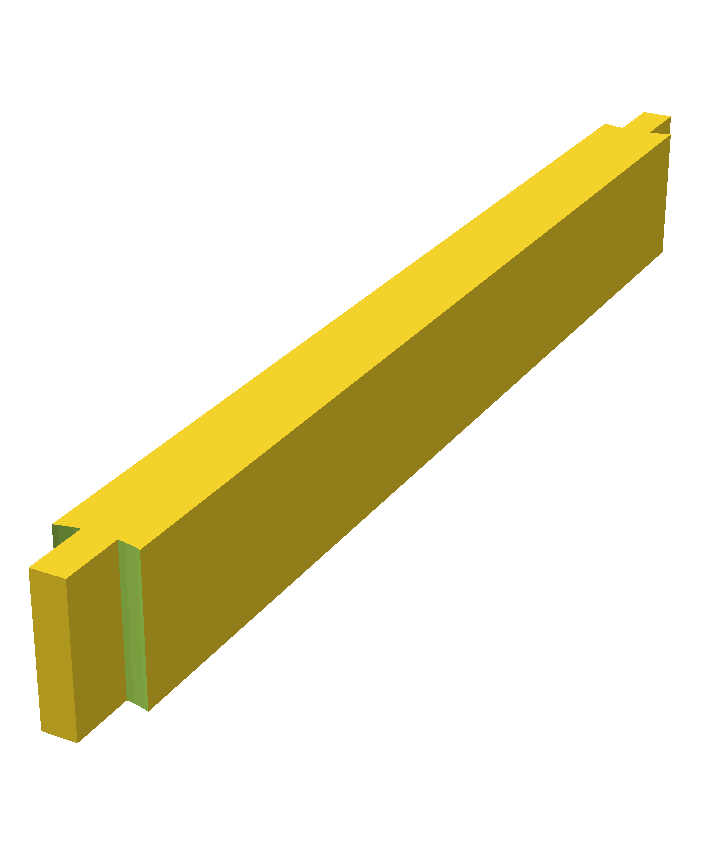
\includegraphics[height=200px, width=240px]{Bilder/Untereinheit_Wand}
\end{Bild}
\todoinline{$\varepsilon$?}

\subsection{Grundplatten}
Grundplatten repräsentieren die Flächen des Grundrisses.
Sie sind aufgebaut aus einem extrudierten Polygon, welches inverse Steckmechanismen am Boden aufweist.
Ein Ausschnitt einer solchen Grundplatte ist in Abbildung 10 zu sehen.
Die inversen Steckmechanismen dienen dem Anbringen der Grundplatte an die Eckpfeiler.
Für jeden Knoten, der an der Fläche anliegt wird hierbei je eine Einkerbung vorgenommen, die auf das Stecksystem des zu dem Knoten zugehörigen Eckpfeiler passt.
%Diese werden durch Differenzen des Ausgangspolygon mit dem negativen komplementären CornerPin realisiert.
%So entsteht für jeden Knoten der Fläche eine Einkerbung für die Verankerung.
\begin{Bild}{Eine Grundplatte (Screenshot der Verfasser)}
	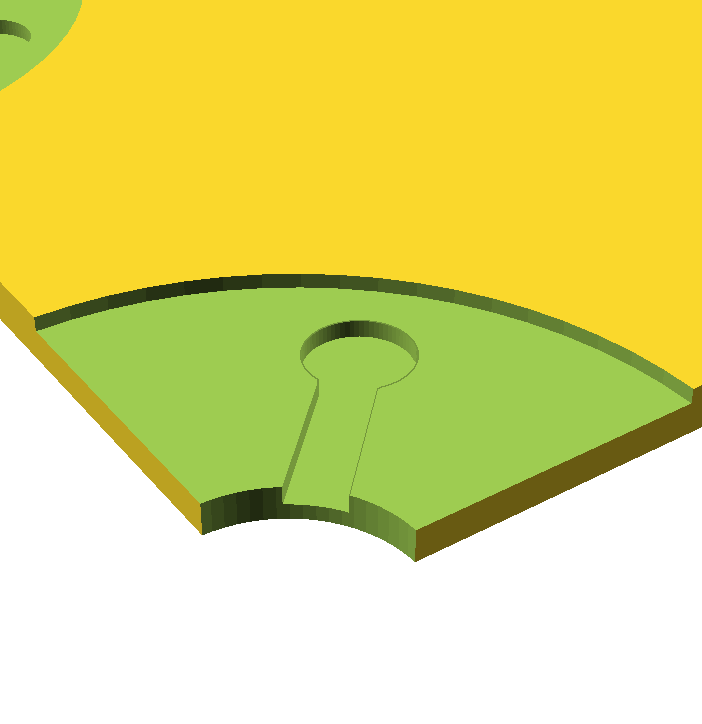
\includegraphics[height=300px]{Bilder/Untereinheit_GP}
\end{Bild}
\todoinline{Abstand zwischen Flächen; Vergrößerung von an das äußere Gebiet angrenzende Fläche}

\subsection{Zuweisen von Berechnungskonstanten}
\subsubsection{Funktion der \icode{Params}-Klasse}
Die \icode{Params}-Klasse wird als statische Zugriffsmöglichkeit auf bestimmte Konstanten des Programms verwendet, welche bei der Berechnung der Bauteile vonnöten sind.
Diese Klasse verfügt hierbei über öffentliche statische Funktionen, mit der aus allen anderen Klassen ohne eine Instanziierung der \icode{Params}-Klasse deren Parameter gesetzt oder auf bereits vorhandene Parameter zugegriffen werden kann.
Die Statik der Variablen und Funktionen verhindert hierbei, dass während des Programmablaufes verschiedene  Berechnungskomponenten unterschiedliche Konstanten zur Verfügung gestellt bekommen. \\
Das Setzen der Parameter findet zu Beginn des Programmes in der \icode{Main}-Klasse statt.
Hierbei wird die Funktion \icode{setParams()} aufgerufen.
Dieser Funktion werden sämtliche Werte als Parameter des Datentyps \icode{double} übergeben.
In der \icode{Params}-Klasse werden dann innerhalb der Funktion allen privaten Variablen ihre Werte entsprechend der Parameter zugewiesen und abrufbar gemacht.\\

\begin{code} [Die \icode{setParams()}-Funktion zum Setzen der Parameter]
	public static void setParams(double E, ...){
		e = E;
		// ...
	}
\end{code}

Das Abrufen der Parameter erfolgt dann mittels der entsprechenden \icode{get()}-Funktionen der \icode{Params}-Klasse, welche für alle Parameter vorhanden sind.
Ein Überschreiben einzelner Parameter wird an dieser Stelle verhindert, da für die privaten Variablen keine \icode{set()}-Funktionen vorliegen.
Der Aufbau der \icode{get()}-Funktionen folgt dem generellen Aufbau des nachfolgenden Codebeispiels, jedoch werden die Parameterbezeichnungen jeweils entsprechend ersetzt:\\

\begin{code} [Die \icode{get()}-Funktion für den Parameter \icode{e}]
public static double getE() {
	return e;
}
\end{code}

Diese Funktionen werden dann aus den Programmteilen, in denen sie für Berechnungen benötigt werden, statisch mittels des Aufrufs der \icode{Params}-Klasse aufgerufen. \\
Die Bedeutung der einzelnen Parameter erklärt sich wie folgt:

\begin{description}[style=nextline]
	\item[E ($\epsilon$/Epsilon)] 
		Der Parameter \q{E} entspricht der Konstante $\epsilon$ (Epsilon), welcher aus Gründen der vorteilhaften Kürze der Parameternamen hier verwendet wurde.
		Somit muss nicht jedes mal \icode{Epsilon} ausgeschrieben werden, es wird auf \icode{E} reduziert.
		$\epsilon$ bezeichnet den Abstand, welcher zwischen zwei Bauteilen mit einberechnet werden muss, um ein einfaches Zusammenstecken zu gewährleisten.
	\item[CornerRadius]
		Der Parameter \q{CornerRadius} entspricht der Konstante, welche den Radius des Grundzylinders der Eckstücken angibt.
	\item[PinMinLength] 
		Der Parameter \q{PinMinLength} entspricht der Konstante, welche die minimale Länge des Quaders des positiven Eckstücks angibt, welcher zwischen dem Eckzylinder und dem Pinzylinder platziert wird.
	\item[PinPWidth] 
		Der Parameter \q{PinPWidth} entspricht der Konstante, welche die Weite für den Quader des positiven Eckstücks angibt, welcher zwischen dem Eckzylinder und dem Pinzylinder platziert wird.
	\item[PinPRadius] 
		Der Parameter \q{PinPRadius} entspricht der Konstante, welche den Radius des Pinzylinders des positiven Eckstücks angibt.
	\item[PinDistance]
		Der Parameter \q{PinDistance} entspricht der Konstante, welche die Distanz zwischen dem positiven Pin und den anliegenden Wandstücken angibt, welche für jeden Pin eingehalten werden muss.
	\item[Height]
		Der Parameter \q{Height} entspricht der Konstante, welche die Höhe der Wandteile und der Eckzylinder angibt.
	\item[PinHeight]
		Der Parameter \q{PinHeight} entspricht der Konstante, welche die Höhe des positiven Pinzylinders angibt.
	\item[BasePlateHeight]
		Der Parameter \q{BasePlateHeight} entspricht der Konstante, welche die Höhe der Grundplatte angibt.
	\item[BasePlatePinCircleHeight]
		Der Parameter \q{BasePlateCircleHeight} entspricht der Konstante, welche die Höhe der Kreisflächen angibt, die unter den positiven Eckstücken angebracht werden und der Stabilisierung und Verankerung von Grundplatter und Eckstück dienen.
\end{description}

\subsection{OpenSCAD Java Interface}
Für die erleichterte Erstellung von OpenScad Objekten wurde ein Java Interface \icode{ScadObject} erstellt, welches alle für das Projekt wichtigen Befehle enthält.
Die Methode \icode{toString()} stellt in den Klassen des Interfaces die Übergabe des OpenSCAD Befehlsstrings dar.
So kann man z.B. mit der Klasse \icode{Cube} einen Quader mit Länge, Höhe und Breite erstellen der dann wie folgt mit \icode{Cube.toString()} in einen String konvertiert wird:
\icode{cube([Länge, Breite, Höhe]);}\\
\begin{Bild}{Resultat der Eingabe: \icode{new Cube(3, 4, 5).toString()} (Screenshot der Verfasser)}
	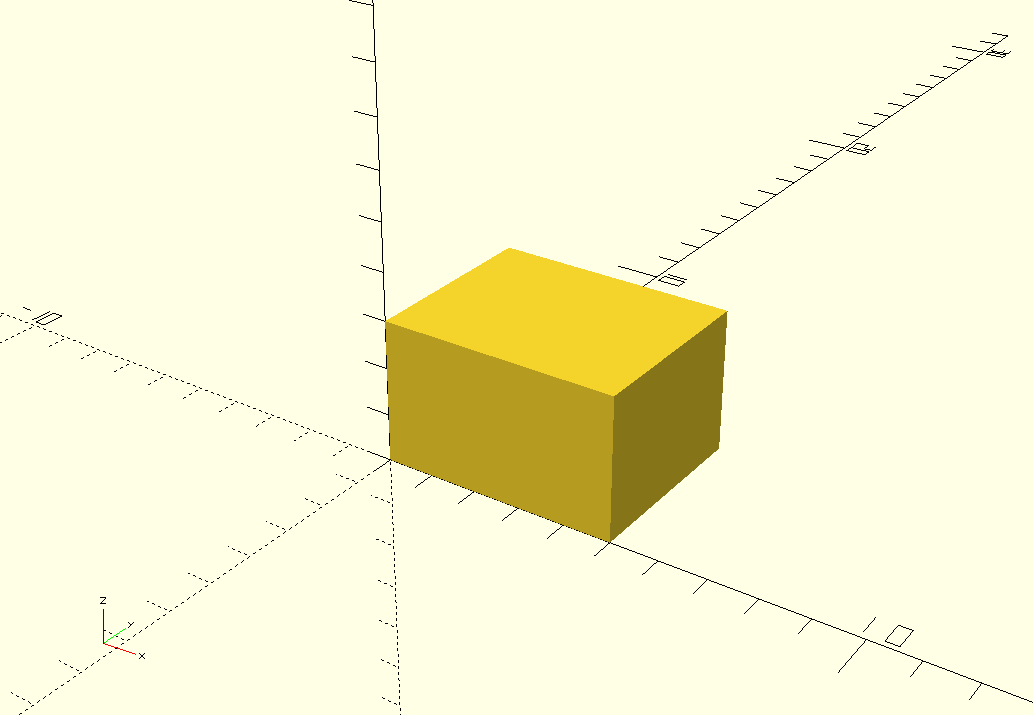
\includegraphics[height = 200px]{Bilder/Quader}
\end{Bild}